%!TEX TS-program = xelatex
%!TEX encoding = UTF-8 Unicode
% @Author: yancz1989
% @Date:   2016-03-29 14:53:26
% @Last Modified by:   yancz1989
% @Last Modified time: 2016-03-31 16:44:20

\documentclass[oneside]{article}
%
% ADD PACKAGES here:
%

\usepackage{mathrsfs}
\usepackage{amsfonts}
\usepackage{indentfirst}
\usepackage{amsmath}
\usepackage{cite}
\usepackage{amssymb}
\usepackage{multirow}
\usepackage{array}
\usepackage{algorithm2e}
\usepackage{xeCJK}
\usepackage{longtable}
\usepackage{graphicx}
\usepackage{subfigure}
\usepackage{geometry}
\usepackage{color}
\usepackage{url}
\usepackage{fancyhdr}
\usepackage{enumitem}
\usepackage{parskip}
\usepackage{hyperref}
\setlength{\oddsidemargin}{0 in}
\setlength{\evensidemargin}{0 in}
\setlength{\topmargin}{-0.6 in}
\setlength{\textwidth}{6.5 in}
\setlength{\textheight}{8.5 in}
\setlength{\headsep}{0.75 in}
\setlength{\parindent}{0 in}
\setlength{\parskip}{5pt}
\setlist[itemize]{parsep=0pt}
\setlist[enumerate]{parsep=0pt}
\linespread{1.4}
\geometry{a4paper}

\usepackage{fontspec,indentfirst}

\setCJKfamilyfont{kaiti}{Kaiti SC Regular}
\newcommand*{\kai}{\CJKfamily{kaiti}} % 楷体_GB2312
\setCJKfamilyfont{heiti}{Heiti SC Light}
\newcommand*{\hei}{\CJKfamily{heiti}} % 黑体
\newcommand*{\song}{\CJKfamily{song}} % 宋体
\setCJKfamilyfont{fangsong}{FangSong}
\newcommand*{\fang}{\CJKfamily{fangsong}}  % 仿宋
\defaultfontfeatures{Mapping=tex-text}

\XeTeXlinebreaklocale "zh"
\XeTeXlinebreakskip=0pt plus 1pt minus 0.1pt

%
% The following commands set up the lecnum (lecture number)
% counter and make various numbering schemes work relative
% to the lecture number.
%
\renewcommand{\thepage}{\arabic{page}}
\renewcommand{\thesection}{\arabic{section}}
\renewcommand{\theequation}{\arabic{section}.\arabic{equation}}
\renewcommand{\thefigure}{\arabic{section}.\arabic{figure}}
\renewcommand{\thetable}{\arabic{section}.\arabic{table}}
\renewcommand{\baselinestretch}{1.4} \normalsize

\DeclareMathOperator*{\argmin}{\arg\!\min}

%
% The following macro is used to generate the header.
\newcommand{\lecture}[5]{
   \newpage
   \noindent
   \begin{center}
        {\LARGE \bf #1} \\
        \vspace{0.5cm}
        {\bf #2} \\
        \vspace{0cm}
        #3\\
        \vspace{0.3cm}
        \it Date: #4
   \end{center}
}
%




% Convention for citations is authors' initials followed by the year.
% For example, to cite a paper by Leighton and Maggs you would type
% \cite{LM89}, and to cite a paper by Strassen you would type \cite{S69}.
% (To avoid bibliography problems, for now we redefine the \cite command.)
% Also commands that create a suitable format for the reference list.
\renewcommand{\cite}[1]{[#1]}
\def\beginrefs{\begin{list}%
        {[\arabic{equation}]}{\usecounter{equation}
         \setlength{\leftmargin}{2.0truecm}\setlength{\labelsep}{0.4truecm}%
         \setlength{\labelwidth}{1.6truecm}}}
\def\endrefs{\end{list}}
\def\bibentry#1{\item[\hbox{[#1]}]}

%Use this command for a figure; it puts a figure in wherever you want it.
%usage: \fig{NUMBER}{SPACE-IN-INCHES}{CAPTION}
\newcommand{\fig}[2]{
            \vspace{#1}
            \begin{center}
            Figure ~#2
            \end{center}
    }
% Use these for theorems, lemmas, proofs, etc.
%
\newcounter{theorem_no}[section]
\newcounter{definition_no}[section]
\newtheorem{theorem}{Theorem}[section]
\newtheorem{lemma}[theorem]{Lemma}
\newtheorem{proposition}[theorem]{Proposition}
\newtheorem{claim}[theorem]{Claim}
\newtheorem{corollary}[theorem]{Corollary}
\newtheorem{definition}[definition_no]{Definition}
\newenvironment{proof}{{\bf Proof:}}{\hfill\rule{2mm}{2mm}}

\newcommand{\homework}[4]{
\pagestyle{myheadings} \thispagestyle{plain}
\newpage
\setcounter{page}{1} \setcounter{section}{#4} \noindent
\begin{center}
\framebox{ \vbox{\vspace{2mm} \hbox to 6.28in { {\bf
THU-70250043,~Pattern~Recognition~(Spring 2016) \hfill Homework: 5} }
\vspace{6mm} \hbox to 6.28in { {\Large \hfill #1 \hfill} }
\vspace{6mm} \hbox to 6.28in { {\it Lecturer: #2 \hfill} }
\vspace{2mm} \hbox to 6.28in { {\it Student: #3 \hfill} }
\vspace{2mm} } }
\end{center}
\markboth{#1}{#1} \vspace*{4mm} }

% **** IF YOU WANT TO DEFINE ADDITIONAL MACROS FOR YOURSELF, PUT THEM HERE:

\newcommand\E{\mathbb{E}}
\begin{document}
\homework{Sparse Learning, SVM and KNN}{Changshui Zhang
\hspace{5mm} {\tt zcs@mail.tsinghua.edu.cn}}{Qingfu Wen \hspace{5mm} {\tt
wqf15@mails.tsinghua.edu.cn } }{8}


\section*{Sparse Learning}
\begin{enumerate}
\item Please briefly describe the geometry reason of sparsity using $\ell_1$ regularized optimization from unit circle diagram in Fig.\ref{fig:fig}. And describe the possible sparsity property of outcome using $\ell_2$ and $\ell_{0.5}$(No proof is needed).
    
\emph{\textbf{SOLUTION:}}\\
    From the Fig.\ref{fig:fig}, we can see that $\ell_1$ norm has some 'corner points' which is on the axis. These points are more likely to be the solution of our problem which are sparse(their coordinate have many 0 since they are one the axis). $\ell_2$ norm does not hold sparsity because all the point on the $\ell_2$'s boundary have the same possibility to be a solution. Thus, $\ell_{0.5}$ have sparsity property. 

\item The famous RIP(restricted isometry property) condition is commonly used in sparse recovery theory which demonstrate following property of sampling matrix $A\in R^{p\times m}$: given $S$ a subset of all columns of $A$ and $s=|S|$ an integer, there exists $\delta_S\in(0,1)$ that for any submatrix $A_S\in R^{p\times s}$ of A and for every $y$,
$$(1-\delta_S)||y||_2^2\leq||A_Sy||_2^2\leq(1+\delta_S)||y||_2^2$$
If $\delta_S$ is small enough, there is overwhelming probability that through sparse learning, we can exactly recovery the original signal. If $A$ is a gaussian random matrix, i.e. each element in the matrix is a random variable from $N(0, 1/p)$, there exist following theorem: set $r=s/m$, and further $$f(r)=\sqrt{m/p}\cdot(\sqrt{r}+\sqrt{2(H(r))}), H(r)=-r\log r-(1-r)\log(1-r)$$, for each $\epsilon>0$, the RIP constant $\delta_S$ for $A$ satisfy:
$$P(1 + \delta_S>[1+(1+\epsilon)f(r)]^2)\leq 2\cdot \exp(-mH(r)\cdot\epsilon/2)$$
Please explain why gaussian random matrix can be chosen as the sampling matrix in sparse learning, i.e., why with a large probability, gaussian random matrix have small RIP constant $\delta_S$.

\begin{figure}
\centering
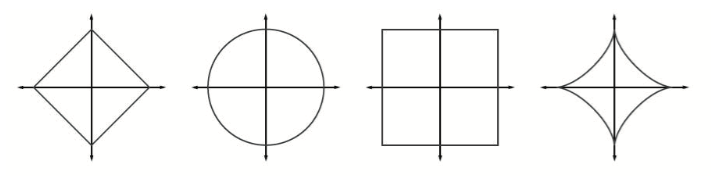
\includegraphics[width=12.5cm]{fig1.png}
\caption{Unit circle of different norms, from left to right: $\ell_1$, $\ell_2$, $\ell_\infty$, and $\ell_{0.5}$}
\label{fig:fig}
\end{figure}

\item You can use MATLAB code from online sources, for example $\ell_1$ Benchmark Package(\url{http://www.eecs.berkeley.edu/~yang/software/l1benchmark/l1benchmark.zip}). Here we recommend using FISTA algorithm, i.e. SolveFISTA.m. Please finish programming to figure out the effectiveness of $\ell_1$ optimization in solving underdetermined systems. You can test the probability of sucessful recovery using simulated data solving $Ax=b$ with different scale of $A$.

\emph{\textbf{SOLUTION:}}\\
suppose $A$ is a $d*n$ matrix and $x$ is a $n*1$ vector with $k$ non-zero elements, then do experiments varying $d,n,k$.
\begin{table}[!htbp]
\centering
\begin{tabular}{|c|c|c|c|}
\hline
 d & n & k & error  \\
\hline
 $8$ & $10$ & $1$ & $9.59*10^{-7}$  \\
\hline
 $80$ & $100$ & $10$ &$ 2.13*10^{-7} $ \\
\hline
$ 800 $&$ 1000 $& $100 $& $2.44*10^{-7}$  \\
\hline
$1600$ & $2000$ & $200$ & $2.04*10^{-7}$ \\
\hline
$2400$ & $3000$ & $300$ & $1.98$ \\
\hline
$8000$ & $10000$ & $1000$ & $3.56 $ \\
\hline
\end{tabular}
\caption{different scale of A}
\end{table}

\end{enumerate}

\section*{SVM}
In this problem, we will use SVM to test on the news20 dataset. We randomly selected 1000 training samples and 1000 testing samples from the whole dataset (For the details of this dataset, refer to \url{https://www.csie.ntu.edu.tw/~cjlin/libsvmtools/datasets/binary.html#news20.binary}). Load the given ".mat" file, \textbf{Xtrn} and \textbf{ytrn} are the training data, \textbf{Xtst} and \textbf{ytst} are the testing data. (\emph{Hint: You can write an SVM yourself, or use the off-the-shelf svm tools such as the libsvm: \url{https://www.csie.ntu.edu.tw/~cjlin/libsvmtools}.})
\begin{enumerate}
\item Train and test SVM with non-linear kernels. Store the parameters that perform best.

\item Train and test linear SVM, compare its performance with the optimal non-linear kernel SVM we get in last step.

\item You can refer to these papers for the details of the SVM tools:

a. C.-C. Chang and C.-J. Lin. LIBSVM : a library for support vector machines. ACM Transactions on Intelligent Systems and Technology, 2:27:1--27:27, 2011.

b. R.-E. Fan, K.-W. Chang, C.-J. Hsieh, X.-R. Wang, and C.-J. Lin. LIBLINEAR: A library for large linear classification Journal of Machine Learning Research 9(2008), 1871-1874.
\end{enumerate}
\emph{\textbf{SOLUTION:}}\\
\begin{table}[!htbp]
\centering
\begin{tabular}{|c|c|}
\hline
 kernel & accuracy  \\
\hline
polynomial & 81.1\%   \\
\hline
radial basis function& 88.5\%\\
\hline
sigmoid & 76.8\% \\
\hline
linear & 88.1\% \\
\hline
\end{tabular}
\caption{different kernel of SVM}
\end{table}
I use \texttt{SVMcgForClass.m} to find parameters $\gamma$ and $c$ with best performance of RBF kernel($c=8,\gamma=0.25$).
\section*{KNN}
Realize KNN classifier yourself, test on mnist dataset and show the experiment results:
\begin{enumerate}
\item Use training datasets with different scales, compare the performances of resulted KNNs, including accuracy, time and space complexity.
\begin{table}[!htbp]
\centering
\begin{tabular}{|c|c|c|c|}
\hline
training size  & accuracy & time & memory \\
\hline
60000 & 0.994 & 582.51 s & 0.39 GB  \\
\hline
30000 & 0.992 & 321.50 s & 0.21 GB  \\
\hline
10000 & 0.992 & 93.79 s & 0.07 GB  \\
\hline
5000 & 0.986 & 48.48 s & 0.04 GB  \\
\hline
2500 & 0.983 & 26.34 s & 0.02 GB  \\
\hline
1000 & 0.977 & 10.83 s & 0.01 GB  \\
\hline
500 & 0.972 &  6.09 s & 0.01 GB  \\
\hline
\end{tabular}
\caption{different training size of kNN}
\end{table}

\item Try KNNs with different k numbers, and compare the performance.
\begin{table}[!htbp]
\centering
\begin{tabular}{|c|c|c|}
\hline
 k & trainSize=1000  & trainSize=10000 \\
\hline
1 & 0.977 & 0.988   \\
\hline
2 & 0.986 & 0.993  \\
\hline
3 & 0.979 & 0.989   \\
\hline
4 & 0.985 & 0.994   \\
\hline
5 & 0.976 & 0.988   \\
\hline
6 & 0.961 & 0.99   \\
\hline
7 & 0.97 & 0.987   \\
\hline
8 & 0.981 & 0.989   \\
\hline
9 & 0.98 & 0.988   \\
\hline
10 & 0.975 & 0.987  \\
\hline
\end{tabular}
\caption{different k of kNN}
\end{table}
\item Try different distance metrics, and compare the performance.
we set $k=3$ and training size$=10000$.
\begin{table}[!htbp]
\centering
\begin{tabular}{|c|c|c|}
\hline
distance metrics & accuracy  \\
\hline
euclidean & 0.989 \\
\hline
cityblock & 0.988 \\
\hline
minkowski & 0.987 \\
\hline
cosine & 0.995   \\
\hline
correlation & 0.993 \\
\hline
jaccard & 0.979 \\
\hline
hamming& 0.91  \\
\hline
\end{tabular}
\caption{different distance metrics of kNN}
\end{table}
\end{enumerate}
\end{document}
